\documentclass[UTF8]{ctexart}
\usepackage{../Zhihu}
\newcommand\low{black!50}
\newcommand\high{green!50}
\title{数字电路学习笔记(十):触发器}
\begin{document}
\maketitle

上一章中提到了普通RS锁存器的两大缺点:

\begin{quote}
\begin{enumerate}
\item $S$端口和$R$端口不能同时有效,但实际应用中不能保证这种情况不出现,此时可能会出错;
\item 在计算机中,有许多内存单元协同组成一个寄存器,存储同一个数据。但每一位数据可能是先后到来的(比如加法器,计算出最高一位会花费比低位更多的时间),如果内存单元被写入的时间无法统一,就会造成混乱。RS锁存器并没有提供控制写入的端口——只要输入变化,状态就会改变。
\end{enumerate}
\end{quote}

本章中将要探讨如何改进这两点,并设计出更加适合存储数据的存储电路。基础电路仍然是RS锁存器:

\begin{figure}
    \begin{circuitikz}[scale=0.7, transform shape]
        \draw (2,2) node[nor port] (not1) {1};
        \draw (2,0) node[nor port] (not2) {2};
        \draw (not1.out) -- ++(1,0) node[right, scale={1/0.7}] {$Q$};
        \draw[green] (not2.out) -- ++(1,0) node[right, scale={1/0.7},black] {$Q'$};
        \draw (not2.in 1) -- ++(-0.3,0);
        \draw[green] (not1.in 2) -- ++(-0.3,0);
        \draw (not1.out)++(0.3,0) to[short,*-] ++(0,-0.7) -- ([shift={(-0.3cm,0.5cm)}]not2.in 1) -- ++(0,-0.5);
        \draw[green] (not2.out)++(0.3,0) to[short,*-,color=green] ++(0,0.7) -- ([shift={(-0.3cm,-0.5cm)}]not1.in 2) -- ++(0,0.5);
        \draw (not1.in 1) -- ++(-1,0) node[left,scale={1/0.7}] {$R$};
        \draw (not2.in 2) -- ++(-1,0) node[left,scale={1/0.7}] {$S$};
    \end{circuitikz}
\end{figure}

\section*{一、门控RS锁存器}

我们从问题二开始解决。为此我们只需增加一个写控制端口。当该端口为高电平时,$S$和$R$可以正常输入;当该端口为低电平时,$S$和$R$被保持在0,锁存器处于保持状态。那么,一个与门便可以解决问题。

\begin{figure}
    \begin{circuitikz}[scale=0.7, transform shape]
        \draw[color=\low] (2,2) node[nor port] (not1) {1};
        \draw[color=\low] (2,0) node[nor port] (not2) {2};
        \draw[color=\low] (not1.out) -- ++(1,0) node[right, scale={1/0.7},color=black] {$Q$};
        \draw[color=\high] (not2.out) -- ++(1,0) node[right, scale={1/0.7},color=black] {$Q'$};
        \draw[color=\low] (not2.in 1) -- ++(-0.3,0);
        \draw[color=\high] (not1.in 2) -- ++(-0.3,0);
        \draw[color=\low] (not1.out)++(0.3,0) to[short,*-] ++(0,-0.7) -- ([shift={(-0.3cm,0.5cm)}]not2.in 1) -- ++(0,-0.5);
        \draw[color=\high] (not2.out)++(0.3,0) to[short,*-] ++(0,0.7) -- ([shift={(-0.3cm,-0.5cm)}]not1.in 2) -- ++(0,0.5);
        \draw (not1.in 1) node[above,color=\low] {$R$} -- ++(-1,0) node[and port, anchor=out] (and1) {};
        \draw (not2.in 2) node[below,color=\low] {$S$} -- ++(-1,0) node[and port, anchor=out] (and2) {};
        \draw (and1.in 2) -- ++(-0.2,0) |- (and2.in 1);
        \draw let \p1=(and1.in 2) in ({\x1-0.2cm},1) to[short,*-] (-3.5,1) node[left,scale={1/0.7}] {$CLK$};
        \draw let \p1=(and1.in 1) in (\x1,\y1) -- (-3.5,\y1) node[left,scale={1/0.7}] {$R$};
        \draw let \p1=(and2.in 2) in (\x1,\y1) -- (-3.5,\y1) node[left,scale={1/0.7}] {$S$};
    \end{circuitikz}
\end{figure}

控制端口,我们将其命名为$CLK$,即时钟(clock)。时钟信号依然是一种普通的信号,只是因为它起控制作用,会周期性变化,所以有这么一个特殊的名字。

门控RS锁存器的功能和普通RS锁存器一样,也有一样的状态转换图和特性方程:$Q^*=S+R'\cdot Q$,唯一不同的就是多了一个控制的时钟信号。当该信号为高时($CLK=1$),锁存器会像普通锁存器一样工作;该信号为低,则无论$S,\,R$输入为什么,状态都会被保持。这样,计算机就可以在时钟为低时做计算,并准备好所有要写入的信号,然后在时钟信号为高时写入。

\section*{二、D锁存器}

接下来,我们解决第一个问题:摆脱RS锁存器的$S\cdot R\neq 1$的约束条件。最简单的解决方法自然是将$S$取反之后作为$R$,这样两者永远不相等,也就不可能都是1了。我们把剩下的一个输入取名为$D$(D是Data的意思——D锁存器是数据存储单元的基础结构)。

\begin{figure}
    \begin{circuitikz}[scale=0.7, transform shape]
        \draw[color=\low] (2,2) node[nor port] (not1) {1};
        \draw[color=\low] (2,0) node[nor port] (not2) {2};
        \draw[color=\low] (not1.out) -- ++(1,0) node[right, scale={1/0.7},color=black] {$Q$};
        \draw[color=\high] (not2.out) -- ++(1,0) node[right, scale={1/0.7}, color=black] {$Q'$};
        \draw[color=\low] (not2.in 1) -- ++(-0.3,0);
        \draw[color=\high] (not1.in 2) -- ++(-0.3,0);
        \draw[color=\low] (not1.out)++(0.3,0) to[short,*-] ++(0,-0.7) -- ([shift={(-0.3cm,0.5cm)}]not2.in 1) -- ++(0,-0.5);
        \draw[color=\high] (not2.out)++(0.3,0) to[short,*-] ++(0,0.7) -- ([shift={(-0.3cm,-0.5cm)}]not1.in 2) -- ++(0,0.5);
        \draw[color=\low] (not1.in 1) node[above,color=\low] {$R$} -- ++(-1,0) node[and port, anchor=out] (and1) {};
        \draw[color=\low] (not2.in 2) node[below,color=\low] {$S$} -- ++(-1,0) node[and port, anchor=out] (and2) {};
        \draw[color=\low] (and1.in 2) -- ++(-0.2,0) |- (and2.in 1);
        \draw[color=\low] let \p1=(and1.in 2) in ({\x1-0.2cm},1) to[short,*-] (-4.5,1) node[left,scale={1/0.7},color=black] {$CLK$};
        \draw let \p1=(and2.in 2) in (\x1,\y1) -- (-4.5,\y1) node[left,scale={1/0.7}] {$D$};
        \draw let \p1=(and1.in 1),\p2=(and2.in 2) in (-4,\y2) to[short,*-] (-4,\y1) node[not port,anchor=in] (not3) {};
        \draw[green] (not3.bout) -- (and1.bin 1);
    \end{circuitikz}
\end{figure}

为此,我们做出的牺牲是放弃了$S=0,\,R=0$时的保持功能。我们可以通过特性方程看它的功能:由于$D=S=R'$,我们有
\[Q^*=D+(D')'\cdot Q=D+D\cdot Q=D\]

因此我们发现,当$CLK=1$时,$Q$会一直和$D$保持同步;然后当$CLK=0$后,才会保持之前的最后一个状态。我们画出它的状态转换图:

\begin{figure}
    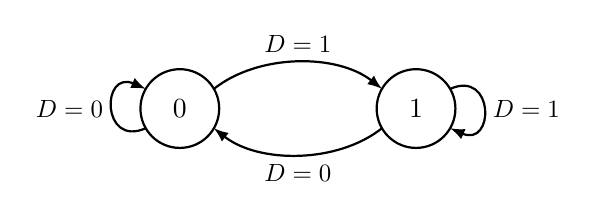
\begin{tikzpicture}
        \tikzset{style={align=center}};
        \draw[thick] (0,0) circle[radius=0.5] node {0};
        \draw[thick,-latex] ([shift={(30:0.5)}]0,0) .. controls (1,0.7) and (2,0.7) .. node[above,scale=0.9] {$D=1$} ([shift={(150:0.5)}]3,0);
        \draw[thick,latex-] ([shift={(-30:0.5)}]0,0) .. controls (1,-0.7) and (2,-0.7) .. node[below,scale=0.9] {$D=0$} ([shift={(-150:0.5)}]3,0);
        \draw[thick,-latex] ([shift={(30:0.5)}]3,0) .. controls (4,0.5) and (4,-0.5) .. node[right,scale=0.9] {$D=1$} ([shift={(-30:0.5)}]3,0);
        \draw[thick,latex-] ([shift={(150:0.5)}]0,0) .. controls (-1,0.5) and (-1,-0.5) .. node[left,scale=0.9] {$D=0$} ([shift={(210:0.5)}]0,0);
        \draw[thick] (3,0) circle[radius=0.5] node {1};
    \end{tikzpicture}
\end{figure}

D锁存器在$CLK=1$时,对输入是“透明”的,和一根导线没有区别;因此,任何输入的变化都会引发状态的变化。其实对于RS锁存器也有这样的问题。但是,这又和我们的第二点设想有冲突:“\textit{内存单元被写入的时间应当统一}”,如果在时钟信号变为低之前,新的数据就已经到来,就会引起错误。究其原因,是因为锁存器能够改变状态的时间是整个高电平期间——为了改进这一点,我们要设法把改变状态的时间缩短为一个时刻。

\section*{三、RS触发器}

一个只在某个时刻发生状态更新的锁存器就叫做触发器。我们考虑如何实现在某个时刻的更新。如果有两个RS锁存器,可以将它们串联,并给一个相反的$CLK$信号:

\begin{figure}
    \begin{circuitikz}[scale=0.7, transform shape]
        \draw[color=\low] (2,2) node[nor port] (not1) {1};
        \draw[color=\low] (2,0) node[nor port] (not2) {2};
        \draw[color=\low] (not2.in 1) -- ++(-0.3,0);
        \draw[color=\high] (not1.in 2) -- ++(-0.3,0);
        \draw[color=\low] (not1.out)++(0.3,0) node[above,color=\low] {$Q_M$} to[short,*-] ++(0,-0.7) -- ([shift={(-0.3cm,0.5cm)}]not2.in 1) -- ++(0,-0.5);
        \draw[color=\high] (not2.out)++(0.3,0) node[below,color=\low] {$Q'_M$} to[short,*-] ++(0,0.7) -- ([shift={(-0.3cm,-0.5cm)}]not1.in 2) -- ++(0,0.5);
        \draw[color=\low] (not1.in 1) node[above,color=\low] {$R_M$} -- ++(-1,0) node[and port, anchor=out] (and1) {};
        \draw[color=\low] (not2.in 2) node[below,color=\low] {$S_M$} -- ++(-1,0) node[and port, anchor=out] (and2) {};
        \draw[color=\low] (and1.in 2) -- ++(-0.2,0) |- (and2.in 1);
        \draw let \p1=(and1.in 2) in ({\x1-0.2cm},1) to[short,*-] (-3.5,1) to[short,-*] (-3.5,-2);
        \draw let \p1=(and1.in 1) in (\x1,\y1) -- (-4,\y1) node[left,scale={1/0.7}] {$R$};
        \draw let \p1=(and2.in 2) in (\x1,\y1) -- (-4,\y1) node[left,scale={1/0.7}] {$S$};
        \draw[color=\low] (10,2) node[nor port] (not3) {1};
        \draw[color=\low] (10,0) node[nor port] (not4) {2};
        \draw[color=\high] (not3.out) -- ++(1,0) node[right, scale={1/0.7},color=black] {$Q'$};
        \draw[color=\low] (not4.out) -- ++(1,0) node[right, scale={1/0.7},color=black] {$Q$};
        \draw[color=\high] (not4.in 1) -- ++(-0.3,0);
        \draw[color=\low] (not3.in 2) -- ++(-0.3,0);
        \draw[color=\high] (not3.out)++(0.3,0) to[short,*-] ++(0,-0.7) -- ([shift={(-0.3cm,0.5cm)}]not4.in 1) -- ++(0,-0.5);
        \draw[color=\low] (not4.out)++(0.3,0) to[short,*-] ++(0,0.7) -- ([shift={(-0.3cm,-0.5cm)}]not3.in 2) -- ++(0,0.5);
        \draw[color=\low] (not3.in 1) node[above,color=\low] {$S_S$} -- ++(-1,0) node[and port, anchor=out] (and3) {};
        \draw[color=\high] (not4.in 2) node[below,color=\low] {$R_S$} -- ++(-1,0) node[and port, anchor=out,color=\low] (and4) {};
        \draw[color=\high] (and3.in 2) -- ++(-0.2,0) |- (and4.in 1);
        \draw (not1.out) -- ++(1,0) |- (and3.in 1) node[above,color=\low] {$S$};
        \draw[color=green] (not2.out) -- ++(1,0) |- (and4.in 2) node[below,color=\low] {$R$};
        \draw (1,-2) node[not port] (not5) {};
        \draw[color=green] let \p1=(and3.in 2) in ({\x1-0.2cm},1) to[short,*-] (4.5,1) -- (4.5,-2) -- (not5.out);
        \draw (not5.in) -- (-4,-2) node[left,scale={1/0.7}] {$CLK$};
    \end{circuitikz}
    \caption*{尤其注意,主锁存器的$Q$要连至从锁存器的$S$,这样才能保持两者状态一致而不是相反}
\end{figure}

第一个锁存器叫主锁存器,第二个叫从锁存器。从锁存器接收主锁存器的状态作为输入。在时钟信号低$\rightarrow$高$\rightarrow$低的一个周期中,它的功能发生了这样的变化:

\begin{enumerate}
\item $CLK=0$时,主锁存器处于保持状态,不接受输入;从锁存器可以工作,但主锁存器状态不改变,所以它也不会发生改变。此时整个触发器就处于保持状态。主锁存器状态为1,则从锁存器$S=1,\,R=0$,状态也为1,反之则状态为0,所以整个触发器的状态和主锁存器状态一致。
\item $CLK=1$时,主锁存器接受输入,能改变状态,但此时从锁存器不再工作,因此该状态改变暂时无法反映到触发器的输出上,触发器仍然处于保持状态;
\item $CLK$又变回0,此时从锁存器重新开始工作,把主锁存器的最后一个状态接收,然后改变触发器输出。
\end{enumerate}

一个信号要想通过整个触发器从输入走到输出,要先在时钟为高时进入主锁存器,然后在变成低电平时从主锁存器进入从锁存器,因此,只有在$CLK$从1变成0的一个瞬间,触发器才会发生状态更新;其他所有时候,都处于保持状态。这被称作下降沿更新。

要做出上升沿更新,也就是$CLK$从0到1的瞬间更新的触发器,只需要让信号在低电平时进入主锁存器,然后在高电平进入从锁存器即可,也就是再加一个反相器:

\begin{figure}
    \begin{circuitikz}[scale=0.7, transform shape]
        \draw[color=\low] (2,2) node[nor port] (not1) {1};
        \draw[color=\low] (2,0) node[nor port] (not2) {2};
        \draw[color=\low] (not2.in 1) -- ++(-0.3,0);
        \draw[color=\high] (not1.in 2) -- ++(-0.3,0);
        \draw[color=\low] (not1.out)++(0.3,0) node[above,color=\low] {$Q_M$} to[short,*-] ++(0,-0.7) -- ([shift={(-0.3cm,0.5cm)}]not2.in 1) -- ++(0,-0.5);
        \draw[color=\high] (not2.out)++(0.3,0) node[below,color=\low] {$Q'_M$} to[short,*-] ++(0,0.7) -- ([shift={(-0.3cm,-0.5cm)}]not1.in 2) -- ++(0,0.5);
        \draw[color=\low] (not1.in 1) node[above,color=\low] {$R_M$} -- ++(-1,0) node[and port, anchor=out] (and1) {};
        \draw[color=\low] (not2.in 2) node[below,color=\low] {$S_M$} -- ++(-1,0) node[and port, anchor=out] (and2) {};
        \draw[color=\high] (and1.in 2) -- ++(-0.2,0) |- (and2.in 1);
        \draw[color=green] let \p1=(and1.in 2) in ({\x1-0.2cm},1) to[short,*-] (-3.5,1) to[short,-*] (-3.5,-2);
        \draw let \p1=(and1.in 1) in (\x1,\y1) -- (-6,\y1) node[left,scale={1/0.7}] {$R$};
        \draw let \p1=(and2.in 2) in (\x1,\y1) -- (-6,\y1) node[left,scale={1/0.7}] {$S$};
        \draw[color=\low] (10,2) node[nor port] (not3) {1};
        \draw[color=\low] (10,0) node[nor port] (not4) {2};
        \draw[color=\high] (not3.out) -- ++(1,0) node[right, scale={1/0.7},color=black] {$Q'$};
        \draw[color=\low] (not4.out) -- ++(1,0) node[right, scale={1/0.7},color=black] {$Q$};
        \draw[color=\high] (not4.in 1) -- ++(-0.3,0);
        \draw[color=\low] (not3.in 2) -- ++(-0.3,0);
        \draw[color=\high] (not3.out)++(0.3,0) to[short,*-] ++(0,-0.7) -- ([shift={(-0.3cm,0.5cm)}]not4.in 1) -- ++(0,-0.5);
        \draw[color=\low] (not4.out)++(0.3,0) to[short,*-] ++(0,0.7) -- ([shift={(-0.3cm,-0.5cm)}]not3.in 2) -- ++(0,0.5);
        \draw[color=\low] (not3.in 1) node[above,color=\low] {$S_S$} -- ++(-1,0) node[and port, anchor=out] (and3) {};
        \draw[color=\high] (not4.in 2) node[below,color=\low] {$R_S$} -- ++(-1,0) node[and port, anchor=out,color=\low] (and4) {};
        \draw[color=\low] (and3.in 2) -- ++(-0.2,0) |- (and4.in 1);
        \draw (not1.out) -- ++(1,0) |- (and3.in 1) node[above,color=\low] {$S$};
        \draw[color=green] (not2.out) -- ++(1,0) |- (and4.in 2) node[below,color=\low] {$R$};
        \draw let \p1=(and3.in 2) in ({\x1-0.2cm},1) to[short,*-] (4.5,1) -- (4.5,-2) -- (not5.out);
        \draw (4.5,-2) -- (2,-2) node[not port,anchor=out] (not7) {};
        \draw[color=green] (not7.bin) -- (-4,-2) node[not port, anchor=bout,color=black] (not9) {};
        \draw (not9.in) -- (-6,-2) node[left,scale={1/0.7}] {$CLK$};
    \end{circuitikz}
\end{figure}

要注意的是,触发器仅仅改变了锁存器更新的机制,并没有改变它的逻辑功能——比如,对于RS触发器,它的特性方程和RS锁存器一致:
\[Q^*=S+R'\cdot Q\]

\section*{四、JK触发器}

对于RS触发器,我们也要继续解决这个约束条件的问题。当然,我们仍可以像D锁存器那样,把$S'$当成$R$;这样连出的电路,自然就是D触发器,将会在后文介绍。

但还有第二种方案,就是利用$Q\oplus Q'=1$的这个性质,将其和$S,\,R$分别相与。不妨管两个输入分别叫$J$和$K$(为了纪念工程师Jack Kilby)——有$S=J\cdot Q',\,R=K\cdot Q$。这样,就必然有$S\cdot R=J\cdot Q'\cdot K\cdot Q=0$。

\begin{figure}
    \begin{circuitikz}[scale=0.7, transform shape]
        \draw[color=\low] (2,2) node[nor port] (not1) {1};
        \draw[color=\low] (2,0) node[nor port] (not2) {2};
        \draw[color=\low] (not2.in 1) -- ++(-0.3,0);
        \draw[color=\high] (not1.in 2) -- ++(-0.3,0);
        \draw[color=\low] (not1.out)++(0.3,0) node[above,color=\low] {$Q_M$} to[short,*-] ++(0,-0.7) -- ([shift={(-0.3cm,0.5cm)}]not2.in 1) -- ++(0,-0.5);
        \draw[color=\high] (not2.out)++(0.3,0) node[below,color=\low] {$Q'_M$} to[short,*-] ++(0,0.7) -- ([shift={(-0.3cm,-0.5cm)}]not1.in 2) -- ++(0,0.5);
        \draw[color=\low] (not1.in 1) node[above,color=\low] {$R_M$} -- ++(-1,0) node[and port, anchor=out] (and1) {};
        \draw[color=\low] (not2.in 2) node[below,color=\low] {$S_M$} -- ++(-1,0) node[and port, anchor=out] (and2) {};
        \draw[color=\low] (and1.in 2) -- ++(-0.2,0) |- (and2.in 1);
        \draw[color=\low] let \p1=(and1.in 2) in ({\x1-0.2cm},1) to[short,*-] (-3,1) to[short,-*] (-3,-2.5);
        \draw[color=\low] let \p1=(and1.in 1) in (\x1,\y1) node[above] {$R$} -- (-3.5,\y1) node[and port, color=black, anchor=out] (and5) {};
        \draw[color=\low] let \p1=(and2.in 2) in (\x1,\y1) node[above] {$S$} -- (-3.5,\y1) node[and port, color=black, anchor=out] (and6) {};
        \draw[color=\low] (10,2) node[nor port] (not3) {1};
        \draw[color=\low] (10,0) node[nor port] (not4) {2};
        \draw[color=\high] (not3.out) -- ++(1,0) node[right, scale={1/0.7},color=black] {$Q'$};
        \draw[color=\low] (not4.out) -- ++(1,0) node[right, scale={1/0.7},color=black] {$Q$};
        \draw[color=\high] (not4.in 1) -- ++(-0.3,0);
        \draw[color=\low] (not3.in 2) -- ++(-0.3,0);
        \draw[color=\high] (not3.out)++(0.3,0) to[short,*-] ++(0,-0.7) -- ([shift={(-0.3cm,0.5cm)}]not4.in 1) -- ++(0,-0.5);
        \draw[color=\low] (not4.out)++(0.3,0) to[short,*-] ++(0,0.7) -- ([shift={(-0.3cm,-0.5cm)}]not3.in 2) -- ++(0,0.5);
        \draw[color=\low] (not3.in 1) node[above,color=\low] {$S_S$} -- ++(-1,0) node[and port, anchor=out] (and3) {};
        \draw[color=\high] (not4.in 2) node[below,color=\low] {$R_S$} -- ++(-1,0) node[and port, anchor=out,color=\low] (and4) {};
        \draw[color=\high] (and3.in 2) -- ++(-0.2,0) |- (and4.in 1);
        \draw[color=\low] (not1.out) -- ++(1,0) |- (and3.in 1) node[above,color=\low] {$S$};
        \draw[color=\high] (not2.out) -- ++(1,0) |- (and4.in 2) node[below,color=\low] {$R$};
        \draw[color=\low] (1,-2.5) node[not port] (not5) {};
        \draw[color=\high] let \p1=(and3.in 2) in ({\x1-0.2cm},1) to[short,*-] (4.5,1) -- (4.5,-2.5) -- (not5.out);
        \draw[color=\low] (not5.in) -- (-6.5,-2.5) node[left,scale={1/0.7},color=black] {$CLK$};
        \draw[color=green] (not3.out)++(0.3,0) -- ++(0,1.5) -- ++(-17.3,0) |- (and6.bin 2);
        \draw[color=black] (not4.out)++(0.3,0) -- ++(0,-1.5) -- ++(-17,0) |- (and5.bin 1);
        \draw[color=black] let \p1=(and5.in 2) in (\x1,\y1) -- (-6.5,\y1) node[left,scale={1/0.7}] {$K$};
        \draw[color=black] let \p1=(and6.in 1) in (\x1,\y1) -- (-6.5,\y1) node[left,scale={1/0.7}] {$J$};
    \end{circuitikz}
\end{figure}

仍然用代入的方法得出它的特性方程:
\[Q^*=S+R'\cdot Q=J\cdot Q'+(K\cdot Q)'\cdot Q=J\cdot Q'+K'\cdot Q\]

但是,这个特性方程不像D锁存器一般直观,所以在画状态转换图时,我们可以分别代入各种输入并列出特性表:

\begin{figure}
    \begin{tabular}{|c|c|c|}\hline\rowcolor{lightgray}
        $J$&$K$&$Q^*$\\\hline
        0&0&$Q$\\\hline
        0&1&0\\\hline
        1&0&1\\\hline
        1&1&$Q'$\\\hline
    \end{tabular}
\end{figure}

从此表来看,J和K的四种取值对应四种功能——其中保持($Q^*=Q$),置1($Q^*=1$),置0($Q^*=0$)三种功能都和RS锁存器对应功能一致,而由于多了$J=K=1$的输入情况,它还有翻转($Q^*=Q'$)的功能。

\begin{figure}
    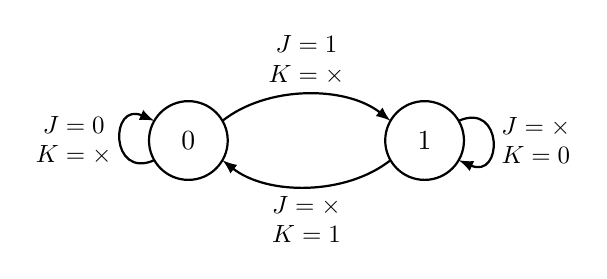
\begin{tikzpicture}
        \tikzset{style={align=center}};
        \draw[thick] (0,0) circle[radius=0.5] node {0};
        \draw[thick,-latex] ([shift={(30:0.5)}]0,0) .. controls (1,0.7) and (2,0.7) .. node[above,scale=0.9] {$J=1$\\$K=\times$} ([shift={(150:0.5)}]3,0);
        \draw[thick,latex-] ([shift={(-30:0.5)}]0,0) .. controls (1,-0.7) and (2,-0.7) .. node[below,scale=0.9] {$J=\times$\\$K=1$} ([shift={(-150:0.5)}]3,0);
        \draw[thick,-latex] ([shift={(30:0.5)}]3,0) .. controls (4,0.5) and (4,-0.5) .. node[right,scale=0.9] {$J=\times$\\$K=0$} ([shift={(-30:0.5)}]3,0);
        \draw[thick,latex-] ([shift={(150:0.5)}]0,0) .. controls (-1,0.5) and (-1,-0.5) .. node[left,scale=0.9] {$J=0$\\$K=\times$} ([shift={(210:0.5)}]0,0);
        \draw[thick] (3,0) circle[radius=0.5] node {1};
    \end{tikzpicture}
\end{figure}

JK触发器相比于RS触发器,还有一个性质,就是它会自己把自己锁死。对于RS锁存器,我们可以放心地在 [公式] 为高电平时随意改变输入,因为从锁存器只关心当它开始工作的一瞬间,也就是 [公式] 下降的那一刻时,主锁存器的状态;但对于JK触发器,我们就不得不关心它在高电平期间的输入,而不只是下降沿瞬间的输入。比如,考虑这样的变化:

\begin{figure}
    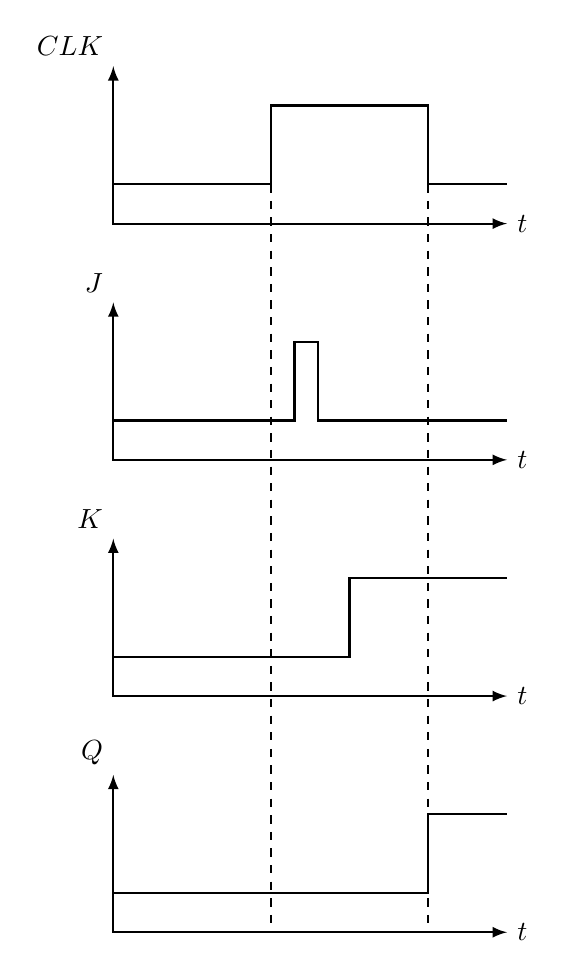
\begin{tikzpicture}
        \draw[thick,latex-latex] (0,5) node[above left] {$CLK$} -- (0,3) -- (5,3) node[right] {$t$};
        \draw[thick,latex-latex] (0,2) node[above left] {$J$} -- (0,0) -- (5,0) node[right] {$t$};
        \draw[thick,latex-latex] (0,-1) node[above left] {$K$} -- (0,-3) -- (5,-3) node[right] {$t$};
        \draw[thick,latex-latex] (0,-4) node[above left] {$Q$} -- (0,-6) -- (5,-6) node[right] {$t$};
        \draw[thick,dashed] (2,3.5) -- (2,-6) (4,3.5) -- (4,-6);
        \draw[thick] (0,3.5) -| (2,4.5) -| (4,3.5) -- (5,3.5);
        \draw[thick] (0,0.5) -| (2.3,1.5) -| (2.6,0.5) -- (5,0.5);
        \draw[thick] (0,-2.5) -| (3,-1.5) -- (5,-1.5);
        \draw[thick] (0,-5.5) -| (4,-4.5) -- (5,-4.5);
    \end{tikzpicture}
\end{figure}

理论上,在高电平期间的$J$的那一个小扰动不应该影响最终的输出——触发器应该在时钟的下降沿工作,而那一刻对应的是$J=0,\,K=1$。因此,$Q$应该保持在0。然而,却发现$Q$变成了1。

这是因为,由于$Q$和$Q'$永远相反,在任意时刻,$J$和$K$中只有一个能够工作——比如在这里,当状态为0时,只有$J$能够产生影响,而$K$的取值则根本不影响主锁存器的状态。这样,一旦$J$为1,主锁存器的状态就被保持在了1,无论$K$的取值为何。这被称作“\textbf{textit{一次翻转}}”——JK触发器在两个下降沿之间的一个周期中,一旦被翻转,就无法被还原。它的原理是,只有与现态相反的输入能起作用——$Q=0$时,$J$起作用;$Q=1$时,$K$起作用。这种问题可能会导致状态受到干扰。

\section*{五、D触发器}

仍然令$R=S'$,便可以得到D触发器。

\begin{figure}
    \begin{circuitikz}[scale=0.7, transform shape]
        \draw[color=\low] (2,2) node[nor port] (not1) {1};
        \draw[color=\low] (2,0) node[nor port] (not2) {2};
        \draw[color=\low] (not2.in 1) -- ++(-0.3,0);
        \draw[color=\high] (not1.in 2) -- ++(-0.3,0);
        \draw[color=\low] (not1.out)++(0.3,0) node[above,color=\low] {$Q_M$} to[short,*-] ++(0,-0.7) -- ([shift={(-0.3cm,0.5cm)}]not2.in 1) -- ++(0,-0.5);
        \draw[color=\high] (not2.out)++(0.3,0) node[below,color=\low] {$Q'_M$} to[short,*-] ++(0,0.7) -- ([shift={(-0.3cm,-0.5cm)}]not1.in 2) -- ++(0,0.5);
        \draw[color=\low] (not1.in 1) node[above,color=\low] {$R_M$} -- ++(-1,0) node[and port, anchor=out] (and1) {};
        \draw[color=\low] (not2.in 2) node[below,color=\low] {$S_M$} -- ++(-1,0) node[and port, anchor=out] (and2) {};
        \draw[color=\low] (and1.in 2) -- ++(-0.2,0) |- (and2.in 1);
        \draw let \p1=(and1.in 2) in ({\x1-0.2cm},1) to[short,*-] (-3.5,1) to[short,-*] (-3.5,-2);
        \draw let \p1=(and1.in 1), \p2=(and2.in 2) in (-4,\y2) to[short,*-] (-4,\y1) node[not port, anchor=in] (not0) {};
        \draw[color=\high] (not0.bout) -- (and1.bin 1);
        \node[above,color=\low] at (and1.in 1) {$R$};
        \draw let \p1=(and2.in 2) in (\x1,\y1) node[below,color=\low] {$S$} -- (-5,\y1) node[left,scale={1/0.7}] {$D$};
        \draw[color=\low] (10,2) node[nor port] (not3) {1};
        \draw[color=\low] (10,0) node[nor port] (not4) {2};
        \draw[color=\high] (not3.out) -- ++(1,0) node[right, scale={1/0.7},color=black] {$Q'$};
        \draw[color=\low] (not4.out) -- ++(1,0) node[right, scale={1/0.7},color=black] {$Q$};
        \draw[color=\high] (not4.in 1) -- ++(-0.3,0);
        \draw[color=\low] (not3.in 2) -- ++(-0.3,0);
        \draw[color=\high] (not3.out)++(0.3,0) to[short,*-] ++(0,-0.7) -- ([shift={(-0.3cm,0.5cm)}]not4.in 1) -- ++(0,-0.5);
        \draw[color=\low] (not4.out)++(0.3,0) to[short,*-] ++(0,0.7) -- ([shift={(-0.3cm,-0.5cm)}]not3.in 2) -- ++(0,0.5);
        \draw[color=\low] (not3.in 1) node[above,color=\low] {$S_S$} -- ++(-1,0) node[and port, anchor=out] (and3) {};
        \draw[color=\high] (not4.in 2) node[below,color=\low] {$R_S$} -- ++(-1,0) node[and port, anchor=out,color=\low] (and4) {};
        \draw[color=\high] (and3.in 2) -- ++(-0.2,0) |- (and4.in 1);
        \draw (not1.out) -- ++(1,0) |- (and3.in 1) node[above,color=\low] {$S$};
        \draw[color=green] (not2.out) -- ++(1,0) |- (and4.in 2) node[below,color=\low] {$R$};
        \draw (1,-2) node[not port] (not5) {};
        \draw[color=green] let \p1=(and3.in 2) in ({\x1-0.2cm},1) to[short,*-] (4.5,1) -- (4.5,-2) -- (not5.out);
        \draw (not5.in) -- (-5,-2) node[left,scale={1/0.7}] {$CLK$};
    \end{circuitikz}
\end{figure}

它的逻辑功能仍然是:

\[Q^*=D\]

相比JK触发器,由于它不使用自身状态作约束,所以不会产生一次翻转的问题。和RS触发器一样,它只关心下降沿瞬间主锁存器的状态。

\section*{六、T触发器}

T触发器是一类偏功能性的触发器——它没有做出任何显著的改进,而只是提供了一种特殊的逻辑功能。我们将同一个输入赋给JK触发器的$J$和$K$:

\begin{figure}
    \begin{circuitikz}[scale=0.7, transform shape]
        \draw[color=\low] (2,2) node[nor port] (not1) {1};
        \draw[color=\low] (2,0) node[nor port] (not2) {2};
        \draw[color=\low] (not2.in 1) -- ++(-0.3,0);
        \draw[color=\high] (not1.in 2) -- ++(-0.3,0);
        \draw[color=\low] (not1.out)++(0.3,0) to[short,*-] ++(0,-0.7) -- ([shift={(-0.3cm,0.5cm)}]not2.in 1) -- ++(0,-0.5);
        \draw[color=\high] (not2.out)++(0.3,0) to[short,*-] ++(0,0.7) -- ([shift={(-0.3cm,-0.5cm)}]not1.in 2) -- ++(0,0.5);
        \draw[color=\low] (not1.in 1) -- ++(-1,0) node[and port, anchor=out] (and1) {};
        \draw[color=\low] (not2.in 2) -- ++(-1,0) node[and port, anchor=out] (and2) {};
        \draw[color=\low] (and1.in 2)  -- ++(-0.2,0) |- (and2.in 1);
        \draw[color=\low] let \p1=(and1.in 2) in ({\x1-0.2cm},1) to[short,*-] (-3,1) to[short,-*] (-3,-2.5);
        \draw[color=\low] let \p1=(and1.in 1) in (\x1,\y1) -- (-3.5,\y1) node[and port, anchor=out] (and5) {};
        \draw[color=\low] let \p1=(and2.in 2) in (\x1,\y1) -- (-3.5,\y1) node[and port, anchor=out] (and6) {};
        \draw[color=\low] (10,2) node[nor port] (not3) {1};
        \draw[color=\low] (10,0) node[nor port] (not4) {2};
        \draw[color=\high] (not3.out) -- ++(1,0) node[right, scale={1/0.7},color=black] {$Q$};
        \draw[color=\low] (not4.out) -- ++(1,0) node[right, scale={1/0.7},color=black] {$Q'$};
        \draw[color=\high] (not4.in 1) -- ++(-0.3,0);
        \draw[color=\low] (not3.in 2) -- ++(-0.3,0);
        \draw[color=\high] (not3.out)++(0.3,0) to[short,*-] ++(0,-0.7) -- ([shift={(-0.3cm,0.5cm)}]not4.in 1) -- ++(0,-0.5);
        \draw[color=\low] (not4.out)++(0.3,0) to[short,*-] ++(0,0.7) -- ([shift={(-0.3cm,-0.5cm)}]not3.in 2) -- ++(0,0.5);
        \draw[color=\low] (not3.in 1) -- ++(-1,0) node[and port, anchor=out] (and3) {};
        \draw[color=\high] (not4.in 2) -- ++(-1,0) node[and port, anchor=out,color=\low] (and4) {};
        \draw[color=\high] (and3.in 2) -- ++(-0.2,0) |- (and4.in 1);
        \draw[color=\low] (not1.out) -- ++(1,0) |- (and3.in 1);
        \draw[color=\high] (not2.out) -- ++(1,0) |- (and4.in 2);
        \draw[color=\low] (1,-2.5) node[not port] (not5) {};
        \draw[color=\high] let \p1=(and3.in 2) in ({\x1-0.2cm},1) to[short,*-] (4.5,1) -- (4.5,-2.5) -- (not5.out);
        \draw[color=\low] (not5.in) -- (-6.5,-2.5) node[left,scale={1/0.7},color=black] {$CLK$};
        \draw[color=\high] (not3.out)++(0.3,0) -- ++(0,1.5) -- ++(-17,0) |- (and5.bin 1);
        \draw[color=\low] (not4.out)++(0.3,0) -- ++(0,-1.5) -- ++(-17,0) |- (and6.bin 2);
        \draw[color=black] (and5.in 2) node[below,color=\low] {$K$} -- ++(-0.3,0) |- (and6.in 1) node[above,color=\low] {$J$};
        \draw[color=black] let \p1=(and5.in 2) in ({\x1-0.3cm},1) to[short,*-] (-6.5,1) node[left,scale={1/0.7}] {$T$};
    \end{circuitikz}
\end{figure}

那么,它的特性方程为:

\[Q^*=J\cdot Q'+K'\cdot Q=T\cdot Q'+T'\cdot Q=T\oplus Q\]

同样画出它的真值表和转换图:

\begin{figure}
    \begin{tabular}{|c|c|}\hline\rowcolor{lightgray}
        $T$&$Q^*$\\\hline
        0&$Q$\\\hline
        1&$Q'$\\\hline
    \end{tabular}
\end{figure}

\begin{figure}
    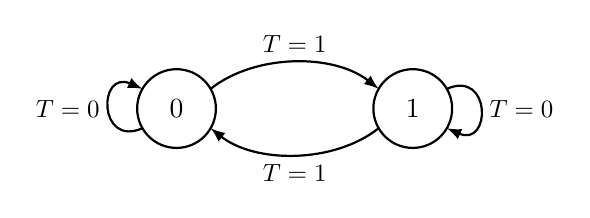
\begin{tikzpicture}
        \tikzset{style={align=center}};
        \draw[thick] (0,0) circle[radius=0.5] node {0};
        \draw[thick,-latex] ([shift={(30:0.5)}]0,0) .. controls (1,0.7) and (2,0.7) .. node[above,scale=0.9] {$T=1$} ([shift={(150:0.5)}]3,0);
        \draw[thick,latex-] ([shift={(-30:0.5)}]0,0) .. controls (1,-0.7) and (2,-0.7) .. node[below,scale=0.9] {$T=1$} ([shift={(-150:0.5)}]3,0);
        \draw[thick,-latex] ([shift={(30:0.5)}]3,0) .. controls (4,0.5) and (4,-0.5) .. node[right,scale=0.9] {$T=0$} ([shift={(-30:0.5)}]3,0);
        \draw[thick,latex-] ([shift={(150:0.5)}]0,0) .. controls (-1,0.5) and (-1,-0.5) .. node[left,scale=0.9] {$T=0$} ([shift={(210:0.5)}]0,0);
        \draw[thick] (3,0) circle[radius=0.5] node {1};
    \end{tikzpicture}
\end{figure}

由此发现,它只有“保持”和“翻转”的功能,也就是JK触发器中$J=K$对应的两个功能。

总结:本文中,我们的锁存器经历了如下的迭代:

\begin{figure}
    \begin{circuitikz}[scale=0.7, transform shape]
        \draw (2,2) node[nor port] (not1) {1};
        \draw (2,0) node[nor port] (not2) {2};
        \draw (not1.out) -- ++(1,0) node[right, scale={1/0.7}] {$Q$};
        \draw[green] (not2.out) -- ++(1,0) node[right, scale={1/0.7},black] {$Q'$};
        \draw (not2.in 1) -- ++(-0.3,0);
        \draw[green] (not1.in 2) -- ++(-0.3,0);
        \draw (not1.out)++(0.3,0) to[short,*-] ++(0,-0.7) -- ([shift={(-0.3cm,0.5cm)}]not2.in 1) -- ++(0,-0.5);
        \draw[green] (not2.out)++(0.3,0) to[short,*-,color=green] ++(0,0.7) -- ([shift={(-0.3cm,-0.5cm)}]not1.in 2) -- ++(0,0.5);
        \draw (not1.in 1) -- ++(-1,0) node[left,scale={1/0.7}] {$R$};
        \draw (not2.in 2) -- ++(-1,0) node[left,scale={1/0.7}] {$S$};
    \end{circuitikz}
    \caption*{RS锁存器}
\end{figure}

\begin{figure}
    \begin{circuitikz}[scale=0.7, transform shape]
        \draw[color=\low] (2,2) node[nor port] (not1) {1};
        \draw[color=\low] (2,0) node[nor port] (not2) {2};
        \draw[color=\low] (not1.out) -- ++(1,0) node[right, scale={1/0.7},color=black] {$Q$};
        \draw[color=\high] (not2.out) -- ++(1,0) node[right, scale={1/0.7},color=black] {$Q'$};
        \draw[color=\low] (not2.in 1) -- ++(-0.3,0);
        \draw[color=\high] (not1.in 2) -- ++(-0.3,0);
        \draw[color=\low] (not1.out)++(0.3,0) to[short,*-] ++(0,-0.7) -- ([shift={(-0.3cm,0.5cm)}]not2.in 1) -- ++(0,-0.5);
        \draw[color=\high] (not2.out)++(0.3,0) to[short,*-] ++(0,0.7) -- ([shift={(-0.3cm,-0.5cm)}]not1.in 2) -- ++(0,0.5);
        \draw (not1.in 1) node[above,color=\low] {$R$} -- ++(-1,0) node[and port, anchor=out] (and1) {};
        \draw (not2.in 2) node[below,color=\low] {$S$} -- ++(-1,0) node[and port, anchor=out] (and2) {};
        \draw (and1.in 2) -- ++(-0.2,0) |- (and2.in 1);
        \draw let \p1=(and1.in 2) in ({\x1-0.2cm},1) to[short,*-] (-3.5,1) node[left,scale={1/0.7}] {$CLK$};
        \draw let \p1=(and1.in 1) in (\x1,\y1) -- (-3.5,\y1) node[left,scale={1/0.7}] {$R$};
        \draw let \p1=(and2.in 2) in (\x1,\y1) -- (-3.5,\y1) node[left,scale={1/0.7}] {$S$};
    \end{circuitikz}
    \caption*{门控RS锁存器}
\end{figure}

\begin{figure}
    \begin{circuitikz}[scale=0.7, transform shape]
        \draw[color=\low] (2,2) node[nor port] (not1) {1};
        \draw[color=\low] (2,0) node[nor port] (not2) {2};
        \draw[color=\low] (not1.out) -- ++(1,0) node[right, scale={1/0.7},color=black] {$Q$};
        \draw[color=\high] (not2.out) -- ++(1,0) node[right, scale={1/0.7}, color=black] {$Q'$};
        \draw[color=\low] (not2.in 1) -- ++(-0.3,0);
        \draw[color=\high] (not1.in 2) -- ++(-0.3,0);
        \draw[color=\low] (not1.out)++(0.3,0) to[short,*-] ++(0,-0.7) -- ([shift={(-0.3cm,0.5cm)}]not2.in 1) -- ++(0,-0.5);
        \draw[color=\high] (not2.out)++(0.3,0) to[short,*-] ++(0,0.7) -- ([shift={(-0.3cm,-0.5cm)}]not1.in 2) -- ++(0,0.5);
        \draw[color=\low] (not1.in 1) node[above,color=\low] {$R$} -- ++(-1,0) node[and port, anchor=out] (and1) {};
        \draw[color=\low] (not2.in 2) node[below,color=\low] {$S$} -- ++(-1,0) node[and port, anchor=out] (and2) {};
        \draw[color=\low] (and1.in 2) -- ++(-0.2,0) |- (and2.in 1);
        \draw[color=\low] let \p1=(and1.in 2) in ({\x1-0.2cm},1) to[short,*-] (-4.5,1) node[left,scale={1/0.7},color=black] {$CLK$};
        \draw let \p1=(and2.in 2) in (\x1,\y1) -- (-4.5,\y1) node[left,scale={1/0.7}] {$D$};
        \draw let \p1=(and1.in 1),\p2=(and2.in 2) in (-4,\y2) to[short,*-] (-4,\y1) node[not port,anchor=in] (not3) {};
        \draw[green] (not3.bout) -- (and1.bin 1);
    \end{circuitikz}
    \caption*{D锁存器}
\end{figure}

\begin{figure}
    \begin{circuitikz}[scale=0.7, transform shape]
        \draw[color=\low] (2,2) node[nor port] (not1) {1};
        \draw[color=\low] (2,0) node[nor port] (not2) {2};
        \draw[color=\low] (not2.in 1) -- ++(-0.3,0);
        \draw[color=\high] (not1.in 2) -- ++(-0.3,0);
        \draw[color=\low] (not1.out)++(0.3,0) node[above,color=\low] {$Q_M$} to[short,*-] ++(0,-0.7) -- ([shift={(-0.3cm,0.5cm)}]not2.in 1) -- ++(0,-0.5);
        \draw[color=\high] (not2.out)++(0.3,0) node[below,color=\low] {$Q'_M$} to[short,*-] ++(0,0.7) -- ([shift={(-0.3cm,-0.5cm)}]not1.in 2) -- ++(0,0.5);
        \draw[color=\low] (not1.in 1) node[above,color=\low] {$R_M$} -- ++(-1,0) node[and port, anchor=out] (and1) {};
        \draw[color=\low] (not2.in 2) node[below,color=\low] {$S_M$} -- ++(-1,0) node[and port, anchor=out] (and2) {};
        \draw[color=\low] (and1.in 2) -- ++(-0.2,0) |- (and2.in 1);
        \draw let \p1=(and1.in 2) in ({\x1-0.2cm},1) to[short,*-] (-3.5,1) to[short,-*] (-3.5,-2);
        \draw let \p1=(and1.in 1) in (\x1,\y1) -- (-4,\y1) node[left,scale={1/0.7}] {$R$};
        \draw let \p1=(and2.in 2) in (\x1,\y1) -- (-4,\y1) node[left,scale={1/0.7}] {$S$};
        \draw[color=\low] (10,2) node[nor port] (not3) {1};
        \draw[color=\low] (10,0) node[nor port] (not4) {2};
        \draw[color=\high] (not3.out) -- ++(1,0) node[right, scale={1/0.7},color=black] {$Q'$};
        \draw[color=\low] (not4.out) -- ++(1,0) node[right, scale={1/0.7},color=black] {$Q$};
        \draw[color=\high] (not4.in 1) -- ++(-0.3,0);
        \draw[color=\low] (not3.in 2) -- ++(-0.3,0);
        \draw[color=\high] (not3.out)++(0.3,0) to[short,*-] ++(0,-0.7) -- ([shift={(-0.3cm,0.5cm)}]not4.in 1) -- ++(0,-0.5);
        \draw[color=\low] (not4.out)++(0.3,0) to[short,*-] ++(0,0.7) -- ([shift={(-0.3cm,-0.5cm)}]not3.in 2) -- ++(0,0.5);
        \draw[color=\low] (not3.in 1) node[above,color=\low] {$S_S$} -- ++(-1,0) node[and port, anchor=out] (and3) {};
        \draw[color=\high] (not4.in 2) node[below,color=\low] {$R_S$} -- ++(-1,0) node[and port, anchor=out,color=\low] (and4) {};
        \draw[color=\high] (and3.in 2) -- ++(-0.2,0) |- (and4.in 1);
        \draw (not1.out) -- ++(1,0) |- (and3.in 1) node[above,color=\low] {$S$};
        \draw[color=green] (not2.out) -- ++(1,0) |- (and4.in 2) node[below,color=\low] {$R$};
        \draw (1,-2) node[not port] (not5) {};
        \draw[color=green] let \p1=(and3.in 2) in ({\x1-0.2cm},1) to[short,*-] (4.5,1) -- (4.5,-2) -- (not5.out);
        \draw (not5.in) -- (-4,-2) node[left,scale={1/0.7}] {$CLK$};
    \end{circuitikz}
    \caption*{RS触发器}
\end{figure}

\begin{figure}
    \begin{circuitikz}[scale=0.7, transform shape]
        \draw[color=\low] (2,2) node[nor port] (not1) {1};
        \draw[color=\low] (2,0) node[nor port] (not2) {2};
        \draw[color=\low] (not2.in 1) -- ++(-0.3,0);
        \draw[color=\high] (not1.in 2) -- ++(-0.3,0);
        \draw[color=\low] (not1.out)++(0.3,0) node[above,color=\low] {$Q_M$} to[short,*-] ++(0,-0.7) -- ([shift={(-0.3cm,0.5cm)}]not2.in 1) -- ++(0,-0.5);
        \draw[color=\high] (not2.out)++(0.3,0) node[below,color=\low] {$Q'_M$} to[short,*-] ++(0,0.7) -- ([shift={(-0.3cm,-0.5cm)}]not1.in 2) -- ++(0,0.5);
        \draw[color=\low] (not1.in 1) node[above,color=\low] {$R_M$} -- ++(-1,0) node[and port, anchor=out] (and1) {};
        \draw[color=\low] (not2.in 2) node[below,color=\low] {$S_M$} -- ++(-1,0) node[and port, anchor=out] (and2) {};
        \draw[color=\low] (and1.in 2) -- ++(-0.2,0) |- (and2.in 1);
        \draw[color=\low] let \p1=(and1.in 2) in ({\x1-0.2cm},1) to[short,*-] (-3,1) to[short,-*] (-3,-2.5);
        \draw[color=\low] let \p1=(and1.in 1) in (\x1,\y1) node[above] {$R$} -- (-3.5,\y1) node[and port, color=black, anchor=out] (and5) {};
        \draw[color=\low] let \p1=(and2.in 2) in (\x1,\y1) node[above] {$S$} -- (-3.5,\y1) node[and port, color=black, anchor=out] (and6) {};
        \draw[color=\low] (10,2) node[nor port] (not3) {1};
        \draw[color=\low] (10,0) node[nor port] (not4) {2};
        \draw[color=\high] (not3.out) -- ++(1,0) node[right, scale={1/0.7},color=black] {$Q'$};
        \draw[color=\low] (not4.out) -- ++(1,0) node[right, scale={1/0.7},color=black] {$Q$};
        \draw[color=\high] (not4.in 1) -- ++(-0.3,0);
        \draw[color=\low] (not3.in 2) -- ++(-0.3,0);
        \draw[color=\high] (not3.out)++(0.3,0) to[short,*-] ++(0,-0.7) -- ([shift={(-0.3cm,0.5cm)}]not4.in 1) -- ++(0,-0.5);
        \draw[color=\low] (not4.out)++(0.3,0) to[short,*-] ++(0,0.7) -- ([shift={(-0.3cm,-0.5cm)}]not3.in 2) -- ++(0,0.5);
        \draw[color=\low] (not3.in 1) node[above,color=\low] {$S_S$} -- ++(-1,0) node[and port, anchor=out] (and3) {};
        \draw[color=\high] (not4.in 2) node[below,color=\low] {$R_S$} -- ++(-1,0) node[and port, anchor=out,color=\low] (and4) {};
        \draw[color=\high] (and3.in 2) -- ++(-0.2,0) |- (and4.in 1);
        \draw[color=\low] (not1.out) -- ++(1,0) |- (and3.in 1) node[above,color=\low] {$S$};
        \draw[color=\high] (not2.out) -- ++(1,0) |- (and4.in 2) node[below,color=\low] {$R$};
        \draw[color=\low] (1,-2.5) node[not port] (not5) {};
        \draw[color=\high] let \p1=(and3.in 2) in ({\x1-0.2cm},1) to[short,*-] (4.5,1) -- (4.5,-2.5) -- (not5.out);
        \draw[color=\low] (not5.in) -- (-6.5,-2.5) node[left,scale={1/0.7},color=black] {$CLK$};
        \draw[color=green] (not3.out)++(0.3,0) -- ++(0,1.5) -- ++(-17.3,0) |- (and6.bin 2);
        \draw[color=black] (not4.out)++(0.3,0) -- ++(0,-1.5) -- ++(-17,0) |- (and5.bin 1);
        \draw[color=black] let \p1=(and5.in 2) in (\x1,\y1) -- (-6.5,\y1) node[left,scale={1/0.7}] {$K$};
        \draw[color=black] let \p1=(and6.in 1) in (\x1,\y1) -- (-6.5,\y1) node[left,scale={1/0.7}] {$J$};
    \end{circuitikz}
    \caption*{JK触发器}
\end{figure}


\begin{figure}
    \begin{circuitikz}[scale=0.7, transform shape]
        \draw[color=\low] (2,2) node[nor port] (not1) {1};
        \draw[color=\low] (2,0) node[nor port] (not2) {2};
        \draw[color=\low] (not2.in 1) -- ++(-0.3,0);
        \draw[color=\high] (not1.in 2) -- ++(-0.3,0);
        \draw[color=\low] (not1.out)++(0.3,0) node[above,color=\low] {$Q_M$} to[short,*-] ++(0,-0.7) -- ([shift={(-0.3cm,0.5cm)}]not2.in 1) -- ++(0,-0.5);
        \draw[color=\high] (not2.out)++(0.3,0) node[below,color=\low] {$Q'_M$} to[short,*-] ++(0,0.7) -- ([shift={(-0.3cm,-0.5cm)}]not1.in 2) -- ++(0,0.5);
        \draw[color=\low] (not1.in 1) node[above,color=\low] {$R_M$} -- ++(-1,0) node[and port, anchor=out] (and1) {};
        \draw[color=\low] (not2.in 2) node[below,color=\low] {$S_M$} -- ++(-1,0) node[and port, anchor=out] (and2) {};
        \draw[color=\low] (and1.in 2) -- ++(-0.2,0) |- (and2.in 1);
        \draw let \p1=(and1.in 2) in ({\x1-0.2cm},1) to[short,*-] (-3.5,1) to[short,-*] (-3.5,-2);
        \draw let \p1=(and1.in 1), \p2=(and2.in 2) in (-4,\y2) to[short,*-] (-4,\y1) node[not port, anchor=in] (not0) {};
        \draw[color=\high] (not0.bout) -- (and1.bin 1);
        \node[above,color=\low] at (and1.in 1) {$R$};
        \draw let \p1=(and2.in 2) in (\x1,\y1) node[below,color=\low] {$S$} -- (-5,\y1) node[left,scale={1/0.7}] {$D$};
        \draw[color=\low] (10,2) node[nor port] (not3) {1};
        \draw[color=\low] (10,0) node[nor port] (not4) {2};
        \draw[color=\high] (not3.out) -- ++(1,0) node[right, scale={1/0.7},color=black] {$Q'$};
        \draw[color=\low] (not4.out) -- ++(1,0) node[right, scale={1/0.7},color=black] {$Q$};
        \draw[color=\high] (not4.in 1) -- ++(-0.3,0);
        \draw[color=\low] (not3.in 2) -- ++(-0.3,0);
        \draw[color=\high] (not3.out)++(0.3,0) to[short,*-] ++(0,-0.7) -- ([shift={(-0.3cm,0.5cm)}]not4.in 1) -- ++(0,-0.5);
        \draw[color=\low] (not4.out)++(0.3,0) to[short,*-] ++(0,0.7) -- ([shift={(-0.3cm,-0.5cm)}]not3.in 2) -- ++(0,0.5);
        \draw[color=\low] (not3.in 1) node[above,color=\low] {$S_S$} -- ++(-1,0) node[and port, anchor=out] (and3) {};
        \draw[color=\high] (not4.in 2) node[below,color=\low] {$R_S$} -- ++(-1,0) node[and port, anchor=out,color=\low] (and4) {};
        \draw[color=\high] (and3.in 2) -- ++(-0.2,0) |- (and4.in 1);
        \draw (not1.out) -- ++(1,0) |- (and3.in 1) node[above,color=\low] {$S$};
        \draw[color=green] (not2.out) -- ++(1,0) |- (and4.in 2) node[below,color=\low] {$R$};
        \draw (1,-2) node[not port] (not5) {};
        \draw[color=green] let \p1=(and3.in 2) in ({\x1-0.2cm},1) to[short,*-] (4.5,1) -- (4.5,-2) -- (not5.out);
        \draw (not5.in) -- (-5,-2) node[left,scale={1/0.7}] {$CLK$};
    \end{circuitikz}
    \caption*{D触发器}
\end{figure}

\begin{figure}
    \begin{circuitikz}[scale=0.7, transform shape]
        \draw[color=\low] (2,2) node[nor port] (not1) {1};
        \draw[color=\low] (2,0) node[nor port] (not2) {2};
        \draw[color=\low] (not2.in 1) -- ++(-0.3,0);
        \draw[color=\high] (not1.in 2) -- ++(-0.3,0);
        \draw[color=\low] (not1.out)++(0.3,0) to[short,*-] ++(0,-0.7) -- ([shift={(-0.3cm,0.5cm)}]not2.in 1) -- ++(0,-0.5);
        \draw[color=\high] (not2.out)++(0.3,0) to[short,*-] ++(0,0.7) -- ([shift={(-0.3cm,-0.5cm)}]not1.in 2) -- ++(0,0.5);
        \draw[color=\low] (not1.in 1) -- ++(-1,0) node[and port, anchor=out] (and1) {};
        \draw[color=\low] (not2.in 2) -- ++(-1,0) node[and port, anchor=out] (and2) {};
        \draw[color=\low] (and1.in 2)  -- ++(-0.2,0) |- (and2.in 1);
        \draw[color=\low] let \p1=(and1.in 2) in ({\x1-0.2cm},1) to[short,*-] (-3,1) to[short,-*] (-3,-2.5);
        \draw[color=\low] let \p1=(and1.in 1) in (\x1,\y1) -- (-3.5,\y1) node[and port, anchor=out] (and5) {};
        \draw[color=\low] let \p1=(and2.in 2) in (\x1,\y1) -- (-3.5,\y1) node[and port, anchor=out] (and6) {};
        \draw[color=\low] (10,2) node[nor port] (not3) {1};
        \draw[color=\low] (10,0) node[nor port] (not4) {2};
        \draw[color=\high] (not3.out) -- ++(1,0) node[right, scale={1/0.7},color=black] {$Q$};
        \draw[color=\low] (not4.out) -- ++(1,0) node[right, scale={1/0.7},color=black] {$Q'$};
        \draw[color=\high] (not4.in 1) -- ++(-0.3,0);
        \draw[color=\low] (not3.in 2) -- ++(-0.3,0);
        \draw[color=\high] (not3.out)++(0.3,0) to[short,*-] ++(0,-0.7) -- ([shift={(-0.3cm,0.5cm)}]not4.in 1) -- ++(0,-0.5);
        \draw[color=\low] (not4.out)++(0.3,0) to[short,*-] ++(0,0.7) -- ([shift={(-0.3cm,-0.5cm)}]not3.in 2) -- ++(0,0.5);
        \draw[color=\low] (not3.in 1) -- ++(-1,0) node[and port, anchor=out] (and3) {};
        \draw[color=\high] (not4.in 2) -- ++(-1,0) node[and port, anchor=out,color=\low] (and4) {};
        \draw[color=\high] (and3.in 2) -- ++(-0.2,0) |- (and4.in 1);
        \draw[color=\low] (not1.out) -- ++(1,0) |- (and3.in 1);
        \draw[color=\high] (not2.out) -- ++(1,0) |- (and4.in 2);
        \draw[color=\low] (1,-2.5) node[not port] (not5) {};
        \draw[color=\high] let \p1=(and3.in 2) in ({\x1-0.2cm},1) to[short,*-] (4.5,1) -- (4.5,-2.5) -- (not5.out);
        \draw[color=\low] (not5.in) -- (-6.5,-2.5) node[left,scale={1/0.7},color=black] {$CLK$};
        \draw[color=\high] (not3.out)++(0.3,0) -- ++(0,1.5) -- ++(-17,0) |- (and5.bin 1);
        \draw[color=\low] (not4.out)++(0.3,0) -- ++(0,-1.5) -- ++(-17,0) |- (and6.bin 2);
        \draw[color=black] (and5.in 2) node[below,color=\low] {$K$} -- ++(-0.3,0) |- (and6.in 1) node[above,color=\low] {$J$};
        \draw[color=black] let \p1=(and5.in 2) in ({\x1-0.3cm},1) to[short,*-] (-6.5,1) node[left,scale={1/0.7}] {$T$};
    \end{circuitikz}
    \caption*{T触发器}
\end{figure}

我们改进了上一章所提及的两个问题,并最终得到了两套解决方案:JK触发器和D触发器。这两个触发器,一个更全面,一个更简单,两个都是在时序电路设计中最常用的触发器。
\end{document}